\documentclass{article}
\usepackage{latexsym}
\usepackage{amssymb,amsmath}
\usepackage{custom2}
\usepackage{graphicx} % for figures
\usepackage{epstopdf} % so can use EPS or PDF figures
\usepackage{caption}
\usepackage{subcaption}
\usepackage{url}
\usepackage{amssymb,amsfonts}
\usepackage[all,arc]{xy}
\usepackage{enumerate}
\usepackage{mathrsfs}
\usepackage{booktabs}
\usepackage[pdftex]{hyperref}
\usepackage{lscape}
\captionsetup{justification=RaggedRight, singlelinecheck=false}
\newcommand{\ra}[1]{\renewcommand{\arraystretch}{#1}}
\newcommand{\argmax}{\text{argmax}}
\newcommand{\Tr}{\text{Tr}}
%\newtheorem{claim}{Claim}

\addtolength{\evensidemargin}{-.5in}
\addtolength{\oddsidemargin}{-.5in}
\addtolength{\textwidth}{1.4in}
\addtolength{\textheight}{1.4in}
\addtolength{\topmargin}{-.5in}


\pagestyle{empty}

\begin{document}
\begin{center}
\Large

\end{center}


\vspace{0pt}

\begin{center}
{\bf \LARGE{Development of a Signaling Network}}
\vspace{10pt}
\\ Eleanor Brush
\\ November 01, 2012
\end{center}

\tableofcontents

%\title{Development of Signaling Network}
%\author{Eleanor Brush}
%\maketitle

\vspace{0pt}
\normalsize
\section{Model as a Stochastic Differential Equation}

\subsection{Derivation of the SDE from microscopic events }
There are three processes that can cause an animal's estimate of its dominance with respect to another to change:
\begin{enumerate}
\item an error can be made so that the animal's estimate randomly changes from one point in time to the next without an external stimulus

\item external observations provide evidence about each animal's dominance, e.g. by fighting each other they gather evidence about their relative strength

\item receiving a signal provides evidence that the receiver is dominant to the signaler

\end{enumerate}
{\bf Assumption:} For now, we will assume that the two animals have access to the same external observations, which would be the case, for instance, if they only gather evidence from fights that they both are engaged in.  We can relax this assumption in the future.

Let $X_t^{(i)}$ denote animal $i$'s estimate of its dominance at time $t$.  We can write down equations describing how these estimates change over time:
\begin{align*}
X_{t+\tau}^{(1)}=X_t^{(1)}+\sum_{i=0}^{N_{e_1}(\tau)}E_i^{(1)}+\sum_{i=0}^{N_f(\tau)}F_i+b_{s_2}S_2(X_t^{(2)},\tau)
\\ X_{t+\tau}^{(2)}=X_t^{(2)}+\sum_{i=0}^{N_{e_2}(\tau)}E_i^{(2)}-\sum_{i=0}^{N_f(\tau)}F_i+b_{s_1}S_1(X_t^{(1)},\tau)
\end{align*} 
where
\begin{itemize}
\item $E_i^{(j)}$ describes the magnitude of an error in estimate for animal $j$, which are identically distributed over time; $N_{e_j}(\tau)$ describes the number of error events in an interval of length $\tau$ so that $\sum_{i=0}^{N_{e_j}(\tau)}E_i^{(j)}$ gives the total magnitude of errors in an interval of length $\tau$

\item $F_i$ describes the magnitude of a piece of external evidence, which are identically distributed over time; $N_f(\tau)$ describes the number of external observations in an interval of length $\tau$ so that $\sum_{i=0}^{N_f(\tau)}F_i$ gives the total magnitude of external evidence in an interval of length $\tau$ (and the evidence gathered changes the animal's estimate in opposite directions, i.e. if a fight is won, one animal's estimate is increased while the other's is decreased by the same amount)

\item $S_j(X_t^{(j)},\tau)$ gives the number of signals emitted by individual $j$ in an interval of length $\tau$ and $b_{s_j}$ describes the boost that each of those signals would give to animal $j+1'$s estimate of its dominance

\end{itemize}
The fact that the two animals are privy to the same external observations is captured by the identity of the second sums in the above equations.  {\bf Assumption:} The above equations assume that $\tau$ is small enough so that $X_t$ does not change significantly enough in the interval $[t,t+\tau)$ that signaling rates would change.  (Error and fighting rates do not depend on the estimates-- another assumption.)  We could write the evidence from signals as a sum over several events in the interval $[t,t+\tau)$ as with errors and observations, but this is equivalent to the formulation above since we assume the size of a signal and the strength of a boost from receiving a signal is constant over time.  

We can now describe the distributions from which these events are drawn:
\begin{itemize}
\item $N_{e_j}(\tau)\sim \scr{P}(r_{e_j},\tau)$
\item $E_i^{(j)}\sim \scr{N}(\mu_{e_j},\sigma^2_{e_j}) \text{ , i.i.d.}$
\item $N_f(\tau)\sim\scr{P}(r_f,\tau)$
\item $F_i\sim\scr{N}(\mu_f,\sigma^2_f) \text{ , i.i.d.}$
\item $S_j(X_t^{(j)},\tau)\sim\scr{P}(f(X_t^{(j)}),\tau)$
\end{itemize}
where $\scr{P}(\lambda,\tau)$ denotes a Poisson process with rate $\lambda$ and $\scr{N}(\mu,\sigma^2)$ denotes a Normal distribution with mean $\mu$ and $\sigma^2$.  $f(x)$ gives the rate (probability) of emitting a signal as a function of the estimate $x$, which is decreasing in $x$.

We now make two approximations:
\begin{enumerate}
\item If $Y_i$, i.i.d., are drawn from some distribution and $N(\tau)\sim\scr{P}(\lambda,\tau)$, then $Z(\tau)=\sum_{i=0}^{N(\tau)}Y_i$ is a compound Poisson process with 
\begin{align*}
\E[Z(\tau)]&=\E[N(\tau)]\E[Y]=\lambda\tau\E[Y]
\\ \text{ and } Var(Z(\tau))&=\E[N(\tau)]\E[Y^2]=\lambda\tau\E[Y^2]
\end{align*}
For computational convenience, we will approximate the distribution of $Z(\tau)$ by $\scr{N}(\lambda\tau\E[Y],\lambda\tau\E[Y^2])$. (HOW VALID IS THIS?)

\item If $\tau$ is big enough that enough events happen, then we can approximate the Poisson process $\scr{P}(\lambda,\tau)$ with $\scr{N}(\lambda\tau,\lambda\tau)$.

\end{enumerate}

This allows us to rewrite our equations for $X_t$ as:

\begin{align*}
X_{t+\tau}^{(1)}&=X_t^{(1)}+Y_{e_1}(\tau)+Y_f(\tau)+b_{s_2}Y_{s_2}(X_t^{(2)}\tau)
\\ X_{t+\tau}^{(2)}&=X_t^{(2)}+Y_{e_2}(\tau)-Y_f(\tau)+b_{s_1}Y_{s_1}(X_t^{(1)}\tau)
\end{align*}
where 
\begin{itemize}
\item $Y_{e_j}(\tau)\sim\scr{N}(r_{e_j}\tau\mu_{e_j},r_{e_j}\tau(\sigma_{e_j}^2+\mu_{e_j}^2))$

\item $Y_f(\tau)\sim N(r_f\tau\mu_f,r_f\tau(\sigma^2_f+\mu_f^2)$

\item $Y_{s_j}(\tau)\sim\scr{N}(f(X_t^{(j+1)})\tau,f(X_t^{(j+1)})\tau)$

\end{itemize}
Finally, if we define the following constants:
\begin{align*}
m_{e_j}&=r_{e_j}\mu_{e_j},
\\ n_{e_j}^2&=r_{e_j}(\sigma_{e_j}^2+\mu_{e_j}^2),
\\ m_f&=r_f\mu_f,
\\ n_f^2&=r_f(\sigma_f^2+\mu_f^2),
\end{align*}
then we get the following equations:
\begin{align*}
X_{t+\tau}^{(1)}&=X_t^{(1)}+\left[m_{e_1}+m_f+b_{s_2}f(X_t^{(2)})\right]\tau+n_f\sqrt{\tau}Z^{(1)}+n_{e_1}\sqrt{\tau}Z^{(2)}+b_{s_2}\sqrt{f(X_t^{(2)})}\sqrt{\tau}Z^{(3)}
\\ X_{t+\tau}^{(2)}&=X_t^{(2)}+\left[m_{e_2}-m_f+b_{s_1}f(X_t^{(1)})\right]\tau-n_f\sqrt{\tau}Z^{(1)}+n_{e_2}\sqrt{\tau}Z^{(4)}+b_{s_1}\sqrt{f(X_t^{(1)})}\sqrt{\tau}Z^{(5)}
\end{align*}
where $Z^{(1)},\dots,Z^{(5)}\sim \scr{N}(0,1),$ i.i.d., which are equivalent to the stochastic differential equations:
\begin{align*}
dX_t^{(1)}&=\left[m_{e_1}+m_f+b_{s_2}f(X_t^{(2)})\right]dt+n_fdW_t^{(1)}+n_{e_1}dW_t^{(2)}+b_{s_2}\sqrt{f(X_t^{(2)})}dW_t^{(3)}
\\ dX_t^{(2)}&=\left[m_{e_2}-m_f+b_{s_1}f(X_t^{(1)})\right]dt-n_fdW_t^{(1)}+n_{e_2}dW_t^{(4)}+b_{s_1}\sqrt{f(X_t^{(1)})}dW_t^{(5)}
\end{align*}
where $W_t^{(1)},\dots,dW_t^{(5)}$ are independent Brownian motions.

We could make a few simplifying assumptions to reduce the number of parameters.  {\bf Assumptions:}
\begin{itemize}
\item $r_{e_1}=r_{e_2}$
\item $\mu_{e_1}=\mu_{e_2}$, and even simpler would be to have both equal $0$ (expected error is $0$)
\item $\sigma^2_{e_1}=\sigma^2_{e_2}$
\item $b_{s_1}=b_{s_2}$ 
\item and combining the above would give $m_{e_1}=m_{e_2}$ and $n_{e_1}=n_{e_2}$
\end{itemize}

\subsection{Evolution of probability distribution over time }
More generally, consider a system
$$ dX_t=a(X_t)dt+\sum_{i=1}^5\sigma_i(X_t)dW_t^{(i)}$$
with $W_t^{(1)},\dots,W_t^{(5)}$ independent Brownian motions.
If $a,\sigma_1,\dots,\sigma_5:\R^2\to\R^2,$ are ``nice" enough functions, and the random variable $X_t$ has a ``nice" enough density function (i.e. $\E[g(X_t)]=\int g(x)p(t,x)dx$ for every bounded measurable function $g$), then according to the Fokker-Planck / Kolmogorov forward equation
\begin{align*}
\frac{\partial p}{\partial t}&=-\sum_{i=1}^2\frac{\partial}{\partial x_i}(a^{(i)}(x)p(t,x))+\frac{1}{2}\sum_{i,j=1}^2\sum_{k=1}^5\frac{\partial^2}{\partial x_i\partial x_j}(\sigma_k^{(i)}\sigma_k^{(j)}p(t,x)
\\ \Rightarrow \frac{\partial p}{\partial t}&=-(m_{e_1}+m_f+b_{s_2}f(x_2))\frac{\partial p}{\partial x_1}-(m_{e_2}-m_f+b_{s_1}f(x_1))\frac{\partial p}{\partial x_2}
\\&+\frac{1}{2}(n_{e_1}^2+n_f^2+b_{s_2}^2f(x_2))\frac{\partial^2 p}{\partial x_1^2}-n_f^2\frac{\partial p}{\partial x_1\partial x_2}+\frac{1}{2}(n_{e_2}^2+n_f^2+b_{s_1}^2f(x_1))\frac{\partial^2 p}{\partial x_2^2}
\end{align*}
using the functions $a$ and $\sigma_i$ as for our particular model.  Note that this requires the function $f:\R\to\R$ be $C^2$.

\subsection{Statistics of the Process WITHOUT Signaling Feedback }
%(See ``The Theory of Stochastic Processes," Cox and Miller.)  Let $p(x_0,x,y_0,y;t)$ be the probability of ending up at $x,y$ at time $t$ given that the process started at $x_0,y_0$.  Then $p$ satisfies the backward equation:
%\begin{align}
%-\frac{\partial}{\partial t}p(x_0,x,y_0,y;t)&=(m_{e_1}+m_f+b_{s_2}f(y_0))\frac{\partial}{\partial x_0}p(x_0,x,y_0,y;t)+(m_{e_1}-m_f+b_{s_2}f(x_0))\frac{\partial}{\partial y_0}p(x_0,x,y_0,y;t) \notag
%\\&+\frac{1}{2}(n_f^2+n_{e_1}^2+b_{s_2}^2f(y_0))\frac{\partial^2}{\partial x_0^2}p(x_0,x,y_0,y;t)+n_f^2\frac{\partial^2}{\partial x_0\partial y_0}p(x_0,x,y_0,y;t) \notag
%\\&+\frac{1}{2}(n_f^2+n_{e_2}^2+b_{s_1}^2f(x_0))\frac{\partial^2}{\partial y_0^2}p(x_0,x,y_0,y;t) \label{back}
%\end{align}
%
%We would like to know the expected time until either estimate reaches the signaling threshold $-T$.  
For simplicity, we start with the case where there is no feedback from signaling to the estimates so that the model becomes
\begin{align*}
dX_t^{(1)}&=\left[m_{e_1}+m_f\right]dt+n_fdW_t^{(1)}+n_{e_1}dW_t^{(2)}
\\ dX_t^{(2)}&=\left[m_{e_2}-m_f\right]dt-n_fdW_t^{(1)}+n_{e_2}dW_t^{(4)}
\end{align*}

This is a simple drift-diffusion model.  We can consider the dynamics of each estimate separately.  We will show results for $X_t^{(1)}$, which follow similarly for $X_t^{(2)}$.  As derived in \cite{Bogacz:2006uq}, the expected time until $X_t^{(1)}$ reaches either $-T$ or $T$ is 
\begin{align*}
\frac{T}{m_e+m_f}\tanh\left(\frac{T(m_e+m_f)}{n_f^2+n_e^2}\right)
\end{align*}
and the probability that $X_t^{(1)}$ reaches $-T$ before it reaches $T$ is
\begin{align*}
\frac{1}{1+\exp\left(\frac{2T(m_e+m_f)}{n_f^2+n_e^2}\right)}
\end{align*}
(assuming $X_t^{(1)}=0$).

The stationary distribution of the estimate will be  (I THINK)
\begin{equation}
X^{(1)}\sim N(\exp((m_{e_1}+m_f)t),\frac{n_f^2+n_e^2}{2}t) \label{ddm_stat}
\end{equation} 

\subsection{Ornstein-Uhlenbeck Variant }
As shown in (\ref{ddm_stat}), both the mean and variance of the distribution of estimates increase with time for a pure drift-diffusion model.  The dynamics are more interesting if the estimates don't just keep increasing or decreasing more or less deterministically.  To add negative feedback and prevent this from happening, we can make the size of an error proportional to the current estimate:
\begin{align*}
dX_t^{(1)}&=\left[m_{e_1}X_t^{(1)}+m_f+b_{s_2}f(X_t^{(2)})\right]dt+n_fdW_t^{(1)}+n_{e_1}dW_t^{(2)}+b_{s_2}\sqrt{f(X_t^{(2)})}dW_t^{(3)}
\\ dX_t^{(2)}&=\left[m_{e_2}X_t^{(2)}-m_f+b_{s_1}f(X_t^{(1)})\right]dt-n_fdW_t^{(1)}+n_{e_2}dW_t^{(4)}+b_{s_1}\sqrt{f(X_t^{(1)})}dW_t^{(5)}
\end{align*}
The Fokker-Planck equation now becomes
\begin{align*}
 \frac{\partial p}{\partial t}&=-(m_{e_1}x_1+m_f+b_{s_2}f(x_2))\frac{\partial p}{\partial x_1}-m_{e_1}p-(m_{e_2}x_2-m_f+b_{s_1}f(x_1))\frac{\partial p}{\partial x_2}-m_{e_2}p
\\&+\frac{1}{2}(n_{e_1}^2+n_f^2+b_{s_2}^2f(x_2))\frac{\partial^2 p}{\partial x_1^2}-n_f^2\frac{\partial p}{\partial x_1\partial x_2}+\frac{1}{2}(n_{e_2}^2+n_f^2+b_{s_1}^2f(x_1))\frac{\partial^2 p}{\partial x_2^2}
\end{align*}
If we ignore signaling feedback for the moment and look for a stationary distribution, we want to solve the equation
\begin{align*}
0&=(m_{e_1}x_1+m_f)\frac{\partial p}{\partial x_1}-m_{e_1}p-(m_{e_2}x_2-m_f)\frac{\partial p}{\partial x_2}-m_{e_2}p
\\&+\frac{1}{2}(n_{e_1}^2+n_f^2)\frac{\partial^2 p}{\partial x_1^2}-n_f^2\frac{\partial p}{\partial x_1\partial x_2}+\frac{1}{2}(n_{e_2}^2+n_f^2)\frac{\partial^2 p}{\partial x_2^2}
\\&=(m_ex+m_f)\frac{\partial p}{\partial x}-(m_ey-m_f)\frac{\partial p}{\partial y}-2m_ep+\frac{1}{2}(n_e^2+n_f^2)\frac{\partial^2 p}{\partial x^2}-n_f^2\frac{\partial p}{\partial x\partial y}+\frac{1}{2}(n_e^2+n_f^2)\frac{\partial^2 p}{\partial y^2}
\\& \text{ if we assume $m_{e_1}=m_{e_2}$}
\end{align*}
We can find a stationary distribution for each estimate individually:
\begin{align}
X^{(1)}& \sim N\left(-\frac{m_f}{m_e},\frac{n_f^2+n_e^2}{-2m_e}\right)\ \label{ou_stat1}
\\ \text{ and } X^{(2)} &\sim N\left(\frac{m_f}{m_e},\frac{n_f^2+n_e^2}{-2m_e}\right) \label{ou_stat2}
\end{align}
and the covariance between the two estimates at steady state is
\begin{align*}
Cov(X^{(1)},X^{(2)})=\frac{-n_f^2}{-2m_e}.
\end{align*}

\section{Analyzing the Model without Stochasticity }
As a first pass, we can ignore the Brownian motion / the noise and treat the model as a dynamical system:

\begin{align*}
\frac{dx}{dt}&=-ex+f+br(y+T)
\\ \frac{dy}{dt}&=-ey-f+br(x+T)
\end{align*}

The isoclines of this system are given by
\begin{align*}
\dot{x}=0 \Rightarrow x&=\frac{f}{e}+\frac{b}{e}r(y+T) 
\\\dot{y}=0 \Rightarrow y&=-\frac{f}{e}+\frac{b}{e}r(x+T)
\end{align*}

The Jacobian of this system is given by
$$J(x,y)=\left(\begin{array}{cccc} 
-e & br'(y+T)
\\ br'(x+T) & -e
\end{array}\right)$$
Letting $\tau=Tr(J(x,y))$ and $\Delta=\text{det}(J(x,y)),$ we see that $\tau=-2e$ and $\Delta=e^2-b^2r'(y+T)r'(x+T)$.  Since $e>0$, $\tau<0$ and any fixed point will be a saddle point, a stable sink, or a stable spiral, depending on the sign of $\Delta$.  
\begin{align*}
\Delta<0 &\Leftrightarrow e^2-b^2r'(y+T)r'(x+T)<0 
\\&\Leftrightarrow e<b\sqrt{r'(y+T)r'(x+T)} \text{ since } e,b, \text{ and } r'(y+T)r'(x+T)\geq0
\\ &\Leftrightarrow \left\{\begin{array}{cccc}
b>0 & \text{ if } e=0
\\ b>2\epsilon e & \text{ if } e>0
\end{array}\right.
\end{align*}
Therefore, if there is a fixed point with $r'(y+T)\neq 0$ and $r'(x+T)\neq 0$ (i.e. the isoclines cross where their slopes are not zero), the fixed point is a saddle and there are two other stable fixed points only if $b>2\epsilon e$.  Figure \ref{basins} shows the basins of attraction for the two stable nodes when the system is bistable.  


\begin{figure}
\begin{center}
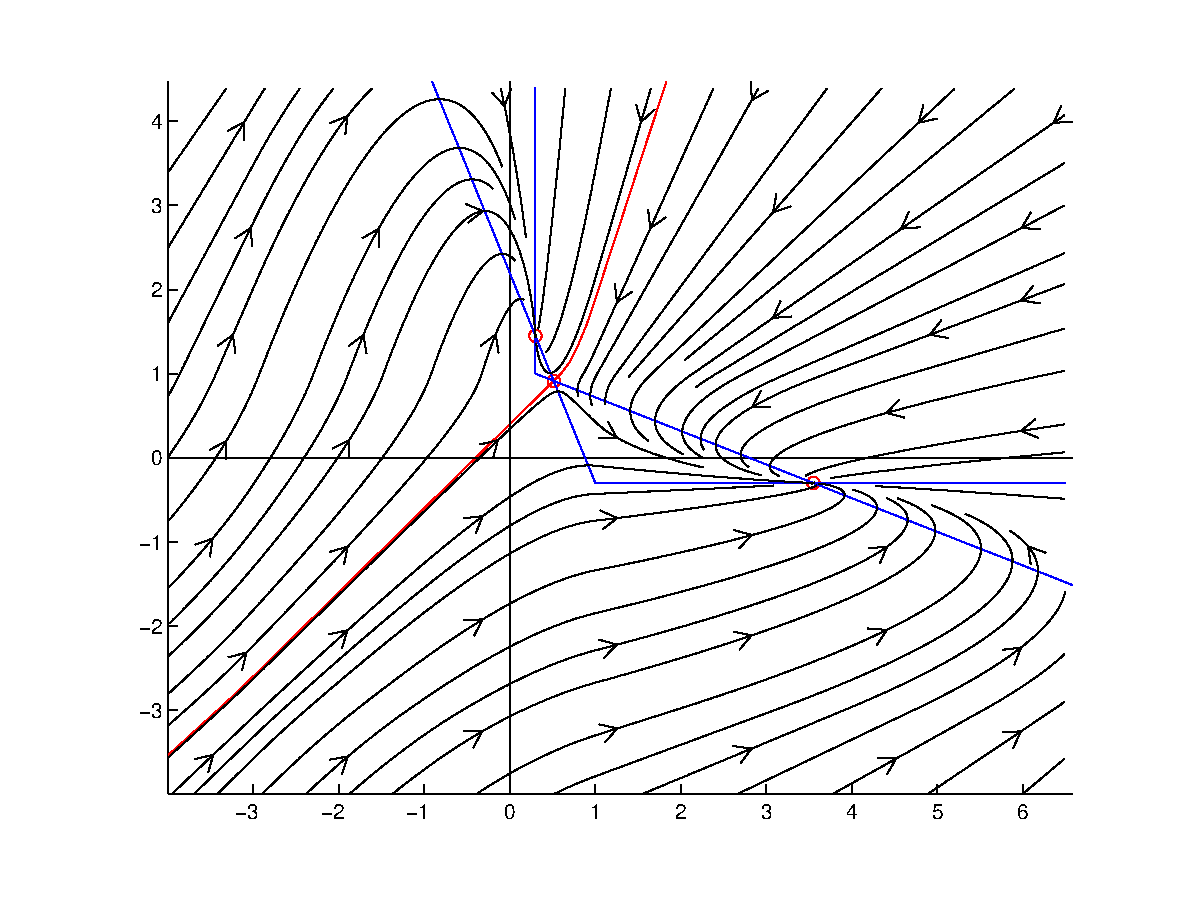
\includegraphics[width=6in]{basins_of_attraction.eps}
\end{center}
\caption{{\bf The basins of attraction for each of the two stable nodes in the case when the system is bistable.} The fixed points are marked in red circles.  The isoclines are marked as blue lines.  The red line separates the basin of attraction for the fixed point where the stronger animal is signaling (above the red line) and the fixed point where the weaker animal is signaling (below the red line). \label{basins}}
\end{figure}


Let $$\psi(b)=\frac{2\epsilon e(\epsilon -\frac{f}{e})-b(\frac{f}{e}+\epsilon)}{2\epsilon e-b} \text{ and } \varphi(b)=\frac{ 2\epsilon e(\epsilon+\frac{f}{e})+b(\frac{f}{e}-\epsilon)}{2\epsilon e-b}$$
Then, there are three general cases, depending on the magnitude of $\frac{f}{e}$ (Figures \ref{bifurcation}-\ref{wireframe}):
\begin{enumerate}
\item $\frac{f}{e}<\epsilon$:
\begin{enumerate}
\item neither animal signaling if $T>\epsilon+\frac{f}{e}$
\item animal 1 not signaling and animal 2 signaling at a non-zero rate if $T<\epsilon+\frac{f}{e}$ and 
$$T>\left\{\begin{array}{cccc}
\varphi(b) & \text{ if } b>2\epsilon e
\\ \psi(b) & \text{ if } b<2\epsilon e
\end{array}\right.$$

\item both animals signal at a non-zero rate if $b<2\epsilon e$ and $T<\psi(b)$
\item two stable equilibria if $b>2\epsilon e$ and $T<\varphi(b)$
\end{enumerate}
\item $\frac{f}{e}>\epsilon$:
\begin{enumerate}
\item neither animal signaling if $T>\epsilon+\frac{f}{e}$
\item animal 1 not signaling and animal 2 signaling at a non-zero rate if $T<\epsilon+\frac{f}{e}$ and $T>\frac{f}{e}-\epsilon$
\item animal 1 not signaling and animal 2 signaling at a rate $=1$ if $T<\frac{f}{e}-\epsilon$
\end{enumerate}
\end{enumerate}
In summary, when the difference in fighting ability is low, there is more uncertainty about which animal is dominant and there can even be two stable equilibria.  Once the difference in fighting ability is great enough, there can never be a stable equilibrium where the stronger animal thinks he is subordinate, but the equilibrium estimate of the weaker animal depends on the threshold below which signaling occurs.

In the above analysis, we considered fixed values of $b$ and $f$ and determined how the value of the threshold $T$ affected the behavior of the system.  In practice, it seems more reasonable for there to be fixed values of $T$ and $b$ (i.e. psychologically all animals in the population are more or less the same), but the difference in fighting ability will vary from pair to pair.  If this is the case, then we need to determine how the value of $f$ affects the behavior of the system (Figures \ref{f_heatmap} and \ref{wireframe}):
\begin{enumerate}
\item $T>\epsilon$ (so that no animal ever signals when he has a positive estimate of its own dominance):
\begin{enumerate}
\item neither animal signals if $f<e(T-\epsilon)$ 
\item the weaker animal signals at a non-zero rate if $f>e(T-\epsilon)$ and $f<e(T+\epsilon)$
\item the weaker animal signals at a maximal rate if $f>e(T+\epsilon)$
\end{enumerate}
\item $T<\epsilon$
\begin{enumerate}
\item both signal if $b<2\epsilon e$ and $f<\frac{(2\epsilon e-b)e(\epsilon-T)}{2\epsilon e+b}$
\item the system is bistable with two equilibria, and in either case one animal doesn't signal and the other signals at a non-zero rate if $b>2\epsilon e$ and $f<\frac{(b-2\epsilon e)e(\epsilon-T)}{2\epsilon e+b}$
\item the weaker animal signals at a non-zero rate if $f>\left|\frac{(b-2\epsilon e)e(\epsilon-T)}{2\epsilon e+b}\right|$ and $f<e(T+\epsilon)$
\item the weaker animal signals at a maximal rate if $f>e(T+\epsilon)$
\end{enumerate}
\end{enumerate}

%\begin{figure}
%\begin{center}
%\includegraphics[width=1\textwidth]{bifurc_diagram.pdf}
%\end{center}
%\caption{{\bf The equilibria of the signaling model as a function of feedback level, $b$, and signaling threshold, $T$.} For both plots, $e=.5$, $\epsilon=.1$. As $f$ increases from less than $\epsilon e$ to greater than $\epsilon e$, the possible equilibria change.  \label{bifurcation}}
%\end{figure}
%
%\begin{figure}
%\begin{center}
%\includegraphics[width=6in]{heatmap_bifurcation_v1.eps}
%\end{center}
%\caption{{\bf The critical value of the parameter $f$ as a function of $b$ and $T$.}  For a given pair of values of $b$ and $T$, if $f$ is above the value indicated by the heatmap the equilibrium of the system is such that the weaker animal signals at a non-zero rate and the stronger animal doesn't signal.  If $f$ is below the value indicated by the heatmap, the equilibria is as indicated by the text. \label{f_heatmap}}
%\end{figure}
%
%\begin{figure}
%%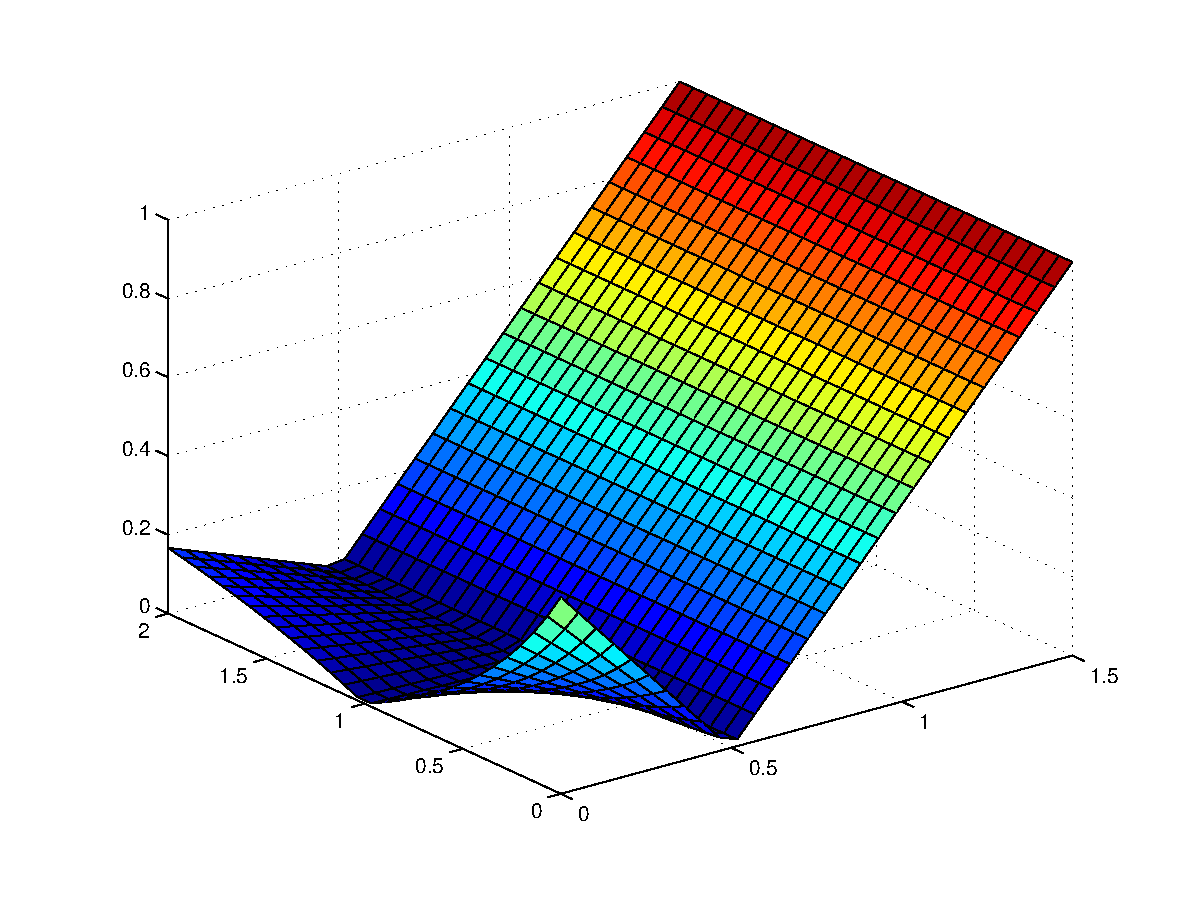
\includegraphics[]{wireframe_bifurcation_v1.eps}
%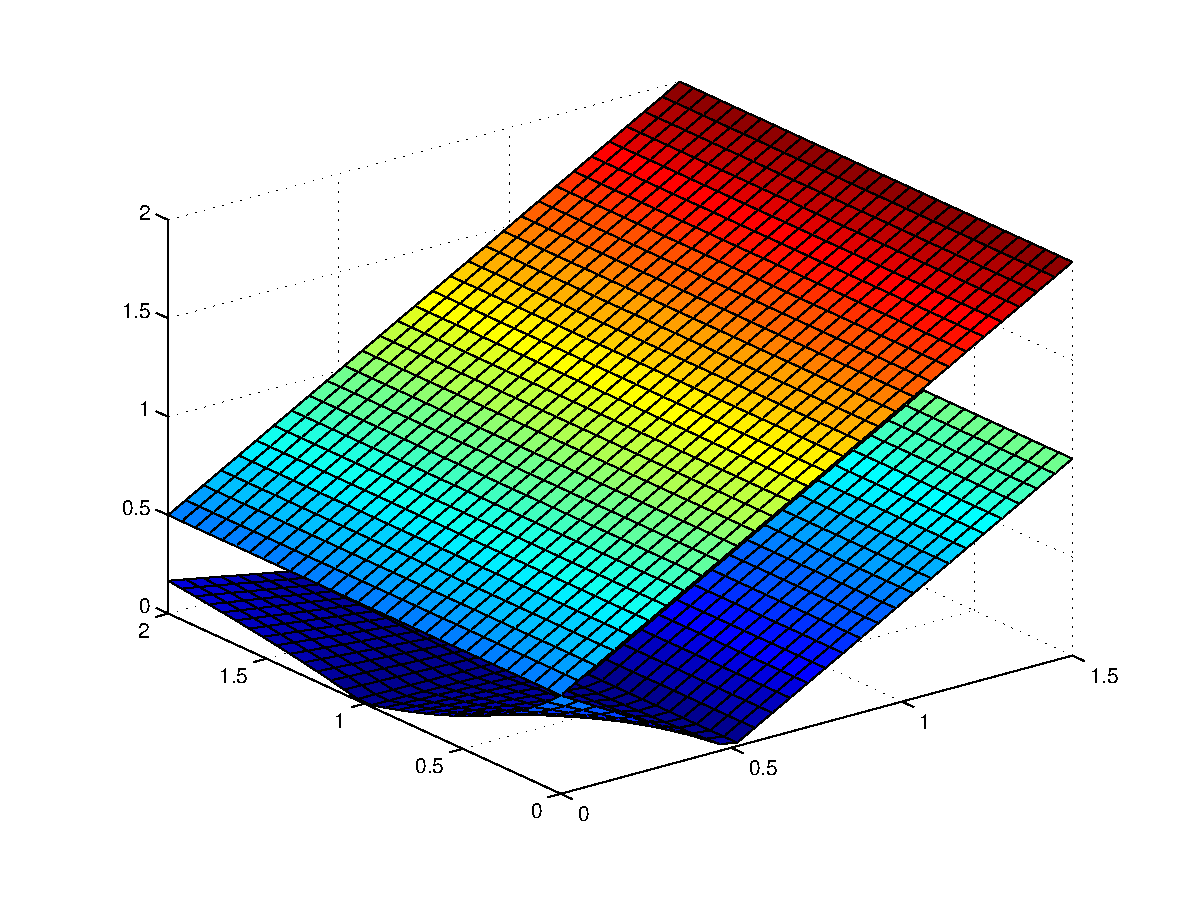
\includegraphics[width=\textwidth]{wireframe_bifurcation_v2.eps}
%\caption{{\bf The dependence of the equilibria of the system on all three parameters, $b$, $T$, and $f$.} $T$ is on the $x$ axis, $b$ is on the $y$ axis and $f$ is on the $z$ axis.  If $f$ is above the upper plane, the equilibrium is such that the weaker animal signals at a maximal rate.  If $f$ is between the two planes, the equilibrium is such that the weaker animal signals at a non-zero rate.  If $f$ is below the lower plane, the equilibria depends on $b$ and $T$ as indicated by Figures \ref{bifurcation} and \ref{f_heatmap}. \label{wireframe}}
%\end{figure}


Suppose these dynamics are going on between every pair of animals in a group where the fighting abilities are drawn from some distribution.  How will a network of signals exchanged develop?  Let's first look at a simple metric of such a network: the number of signalers sending signals to a given animal.  
\begin{align*}
P(n \text{ signalers})=\int P(x)P(n \text{ signalers}|x)dx \text{ where $x$ is the fighting ability of a focal animal}
\end{align*}
If $T>\epsilon$ then animal $i$ signals to animal $j$ if and only if $f_j-f_i>e(T-\epsilon)$.  Therefore,
\begin{align*}
P(n \text{ signalers}|x)={N-1 \choose n}P(x-y>e(T-\epsilon))^nP(x-y<e(T-\epsilon))^{(N-1-n)}
\end{align*}
where $N$ is the total number of animals in the group and we use the binomial distribution to express the probability of $n$ signalers as a function of the probability of one of the other $N-1$ animals signaling, which we assume to be independent events.

At first, we will assume that fighting ability is drawn uniformly from some range $[-L,L]$.  In order for signaling to be possible, we need $e(T-\epsilon)<2L$.
\begin{align*}
\\ \Rightarrow P(x-y>e(T-\epsilon))&=\frac{L+x-e(T-\epsilon)}{2L} \\ \text{ and } P(x-y<e(T-\epsilon))&=\frac{L-x+e(T-\epsilon))}{2L}
\\ \Rightarrow P(n \text{ signalers}|x)&={N-1\choose n}\left(\frac{L+x-e(T-\epsilon)}{2L}\right)^n\left(\frac{L-x+e(T-\epsilon))}{2L}\right)^{(N-1-n)}
\\ \Rightarrow P(n \text{ signalers})&=\int_{-L+e(T-\epsilon)}^L\frac{1}{2L}{N-1\choose n}\left(\frac{L+x-e(T-\epsilon)}{2L}\right)^n\left(\frac{L-x+e(T-\epsilon))}{2L}\right)^{(N-1-n)}dx
\\ &=\int_0^{1-\frac{e(T-\epsilon)}{2L}}{N-1\choose n}z^n(1-z)^{(N-1-n)}dz \text{ using $z=\frac{L+x-e(T-\epsilon)}{2L}$}
\\ &={N-1\choose n}\int_0^{1-\frac{e(T-\epsilon)}{2L}}z^n(1-z)^{(N-1-n)}
\\ &={N-1 \choose n} B\left(1-\frac{e(T-\epsilon)}{2L};n+1,N-n\right) \text{ where $B(c;x,y)=\int_0^cz^{x-1}(1-z)^{y-1}dz$}  
\\&={N-1\choose n}B(n+1,N-n)F\left(1-\frac{e(T-\epsilon)}{2L};n+1,N-n\right)
\\&=\frac{1}{N}F\left(1-\frac{e(T-\epsilon)}{2L};n+1,N-n\right) \tag{$\star$} \label{STAR}
\end{align*} 
where $F(x;\alpha,\beta)=\int_0^x\frac{z^{\alpha-1}(1-z)^{\beta-1}}{B(\alpha,\beta)}dz$ is the cumulative distribution function of the Beta distribution and $B$ is the Beta function with shape parameters $\alpha$ and $\beta$.

If $n=0$, we have to make a small correction:
\begin{align*}
P(0 \text{ signalers})&=\frac{1}{N}F\left(1-\frac{e(T-\epsilon)}{2L};1,N\right)+\frac{e(T-\epsilon)}{2L}
\end{align*}
since if $x\in [-L,-L+\frac{e(T+\epsilon)}{2L}],$ the animal will receive no signals.

Suppose $T=\epsilon$ so signaling at a non-zero rate starts as soon as an animal's estimate is negative.  Then 
\begin{align*}
P(n \text{ signalers})&=\frac{1}{N}F(1-0;n+1,N-n)
\\&=\frac{1}{N}F(1;n+1,N-n)
\\&=\frac{1}{N}
\end{align*}
so the distribution of number of signalers is uniform over the possibilities $0,1,\dots,N-1$.  If $T\gneq \epsilon$, having fewer signalers is more probable and having more signalers is less probably.  The probability distribution of number of signalers for a small set of parameters is shown in Figure \ref{derived_sig_probs}.

\begin{figure}
\includegraphics[width=6in]{distributions_of_signals_received_uniform.pdf}
\caption{The probability distribution of number of signalers, assuming a uniform distribution of fighting abilities, as derived in Eq. (\ref{STAR}).  \label{derived_sig_probs}}
\end{figure}

\section{Simulating the Stochastic Process }
A simple updating algorithm allows us to simulate the process as described by the model above (ORNSTEIN-UHLENBECK VARIANT):

\noindent Fix $\Delta t>0$.  Set $t=0$ and initialize $X_0^{(1)}=X_0^{(2)}=0$.

\begin{enumerate}
\item Draw $Z_1,\dots,Z_5$ i.i.d. from $N(0,1)$.
\item \begin{align*}
X_{t+\Delta t}^{(1)}&=X_t^{(1)}+\left(m_{e_1}X_t^{(1)}+m_f+b_{s_2}f(X_t^{(2)}\right)\Delta t+n_f\sqrt{\Delta t}Z_1+n_{e_1}\sqrt{\Delta t}Z_2+b_{s_2}\sqrt{f(X_t^{(2)}}\sqrt{\Delta t}Z_3\\
X_{t+\Delta t}^{(2)}&=X_t^{(2)}+\left(m_{e_2}X_t^{(2)}+m_f+b_{s_1}f(X_t^{(1)}\right)\Delta t+n_f\sqrt{\Delta t}Z_1+n_{e_2}\sqrt{\Delta t}Z_4+b_{s_1}\sqrt{f(X_t^{(1)}}\sqrt{\Delta t}Z_5
\end{align*}
\item $t=t+\Delta t$


\end{enumerate}

To confirm that our simulation is performing reasonably, we let the model run without signaling feedback until the estimates reach stationary distributions and compare these to the analytical prediction, as given by (\ref{ou_stat1}) and (\ref{ou_stat2}).  This comparison is shown in Figure \ref{ou_stat_dist}.  As can be seen in the figure, the observed probability distribution of estimates is statistically indistinguishable from the prediction (for the first, K-S test $D=0.0243$, $p=0.5969$ and for the second, $D=0.0211$, $p=0.766$).

\begin{figure}
\begin{center}
\includegraphics[width=.65\textwidth]{ou_stat_distribution.pdf} \end{center}
\caption{\label{ou_stat_dist} A comparison between the stationary distribution from a simulation of the Ornstein-Uhlenbeck model and the analytically predicted stationary distribution.}
\end{figure}

We are interested in the effect of signaling feedback, i.e. the $b_s$ parameter, on the dynamics of the model.  We run the algorithm $1000$ times so that we obtain, at each point in time, a distribution of each animal's estimates.  We then compare these distributions when there is and isn't signaling.  In both regimes, each animal's estimates reach a relatively stationary distribution fairly quickly so that we can pick a typical time point at which the distributions are not changing any more.  (A Kolmogorov-Smirnov test for the differences between distributions at different points in time does not allow us to reject the null hypothesis that the distributions are the same, at a significance level of $p=0.05$.)  If we allow the simulation to reach a stationary state, we find that the stationary distributions with and without signaling feedback ($b_{s_1}=b_{s_2}=0$ and $b_{s_1}=b_{s_2}\gneq 0$) are quite different for Animal 1(K-S test statistic, $D=0.995,p<2.2\times10^{-16}$), whereas they are statistically indistinguishable for Animal 2 ($D=0.048, p=0.1995$) (Figure (\ref{diff_dists})).   


By comparing distributions of the estimates at a given point in time, we compare the behavior of the stochastic process over many realizations.  We can also compare the behavior of individual trajectories over time.  We hypothesize that by increasing the strength of signaling feedback, we should increase the stability of signaling behavior and it should be less likely that the dominant animal's estimate sink to such an extent that it becomes subordinate.  To test this hypothesis, we count, for each run of the simulation, the number of switches between dominance regimes.  A dominance regime is defined by one animal's estimate being below the signaling threshold $-T$ and the other animal's estimate being above the positive threshold $T$.  If a dominance regime is established with Animal $i$'s estimate above the threshold (dominant) and Animal $i+1$'s estimate below the threshold (subordinate) and subsequently a dominance regime is established with Animal $i$ subordinate and Animal $i+1$ dominant, we count this as one switch.  Fixing the other parameters of the model, for each difference in fighting ability $m_f$ and level of signaling feedback $b_{s_1}=b_{s_2}$, we can find the average number of switches that occur in a run of the model.  As the difference in fighting ability increases fewer switches occur since Animal 1 is dominant the vast majority of the time.  Additionally, the average number of switches between dominance regimes decreases as $b_{s}$ increases, and the effect is greater for when the difference in fighting ability is smaller (Figure \ref{diff_switches}).
  
\begin{figure}
%\begin{subfigure}{.5 \textwidth}
\begin{center}
\includegraphics[width=.85\textwidth]{feedback_estimate_distributions_v2.pdf}
\end{center}
%\caption{}
%\end{subfigure}
\caption{\label{diff_dists} The distribution of estimates for each animal at time $200$, for no signaling feedback and for signaling feedback $b_{s_1}=b_{s_2}=3$.  Other parameters are set as follows: threshold $T=5$, $m_{e_1}=m_{e_2}=-.5$, $n_{e_1}=n_{e_2}=1$, $m_f=5$, $n_f=.5$. }
\end{figure}

\begin{figure}
\begin{subfigure}{1 \textwidth}
\includegraphics[width=.5\textwidth]{feedback_stability_of_dominance_v2.pdf}
\includegraphics[width=.5\textwidth]{feedback_stability_of_dominance_v5.pdf}
\caption{\label{low_error}}
\end{subfigure}
\begin{subfigure}{1 \textwidth}
\includegraphics[width=.5\textwidth]{feedback_stability_of_dominance_v4.pdf}
\caption{\label{high_error}}
\end{subfigure}
%\begin{subfigure}{.5 \textwidth}
%\includegraphics[width=1\textwidth]{feedback_stability_of_dominance_v2.pdf}
%\caption{}
%\end{subfigure}
\caption{\label{diff_switches} The average number of switches between dominance regimes as a function of the difference in fighting ability, $m_f$, between the animals and the degree to which receiving a signal affects an animal's estimate of its dominance, $b_{s_1}=b_{s_2}$.  In general, even for small differences in fighting ability there are very few switches in dominance regimes.  However, fighting ability can be made small enough to allow switches to occur, in which case the strength of signaling feedbacks affects how frequently they happen.  When the leak rate is relatively low, increases in signaling feedback decrease the number of switches (\ref{low_error}).  When the error rate is high / estimates leak back to $0$ very quickly, increasing the signaling feedback actually increases the number of switches between dominance regimes / decreases the stability of a dominance regime (\ref{high_error}).}
\end{figure}

\section{Linear Learning Formulation}

So far, we have considered how the processes of engaging in fights and sending and receiving signals might affect the estimates two animals make of each other's dominance.  We are interested in understanding these processes on the population level and therefore would like to embed these dynamics in a model of a social network.  In order to make this more analytically tractable, we modify our model into a linear learning model and, for the moment, ignore feedback from signaling into the learning process.  Our main question is how the structure of a social network can facilitate individuals' learning about the states of other nodes in the network.

Suppose each individual has a true fighting ability $a_1,\dots,a_N$ and let $f_{jk}=a_j-a_k$.  Consider an individual in a social network observing its own interactions with other members of the group and the interactions between other members of the group and trying to learn each individual's true fighting ability.  Let $x_j(t)$ be the individual's estimate of individual $j$'s fighting ability at time $t$.  The focal individual will be able to learn about other individual's fighting ability by engaging in fights with individuals it interacts with and observing fights between pairs of individuals both of whom it interacts with.  Let 
$$I_{jk}=\left\{
\begin{array}{cccc}
1 & , & \text{ if the focal individual interacts with both $j$ and $k$}\\
0 & , & \text{ otherwise}
\end{array}\right..
$$
Now, $x_j$ will change according to
\begin{align*}
\dot{x}_j(t)&=\sum_kI_{jk}\left[f_{jk}-(x_j(t)-x_k(t))\right] \text{ for } j\lneq N
\\ \text{ and } x_N(t)&=T-\sum_{j\lneq N}x_j(t),
\end{align*}
where we impose a total on the estimates so that they do not diverge.  Therefore,
\begin{align*}
\dot{x}_j(t)&=\sum_{k\neq N}I_{jk}\left[f_{jk}-(x_j(t)-x_k(t))\right]+I_{jN}\left[f_{jN}-(x_j(t)-x_N(t))\right]
\\&=\sum_{k\neq N}I_{jk}\left[f_{jk}-(x_j(t)-x_k(t))\right]+I_{jN}\left[f_{jN}-(x_j(t)-(T-\sum_{k\neq N}x_k(t)))\right]
\\&=\sum_kI_{jk}f_{jk}-x_j(t)\sum_{k}I_{jk}+\sum_{k\neq N}I_{jk}x_k(t)+TI_{jN}-\sum_{k\neq N}I_{jN}x_k(t)
\\&=\sum_kI_{jk}f_{jk}+TI_{jN}-x_j(t)\sum_kI_{jk}+\sum_{k\neq N}(I_{jk}-I_{jN})x_k(t)
\\&=C_j+\sum_{k}L_{jk}x_k(t) \text{ where } C_j=\sum_{k\neq N}I_{jk}f_{jk}+TI_{jN} \text{ and } 
\end{align*}
$L_{jk}$  is an $n-1\times n-1$ matrix given by
$$
L_{jk}=\left\{
\begin{array}{cccc}
-\sum_lI_{jl}+I_{jj}-I_{jN} & , & \text{ if }j=k
\\ I_{jk}-I_{jN} & , & \text{ if } j\neq k
\end{array}\right..
$$
If $x_k(t)=a_k+\frac{T-\sum_ka_k}{N}$  for all $k$, $\dot{x}(t)=0$.  (If $T=\sum_ka_k$ then $x_k(t)=a_k$ is an equilibrium.)

Stability of the equilibrium is determined by the eigenvalues of $L$.

\section{To Do }

\begin{itemize}
\item More mathematical analysis.
\begin{itemize}
\item We know that if signaling is constantly present or absent, the stationary distribution of the Ornstein-Uhlenbeck process is just shifted and the variance does not change.  However, we do not know what the likelihood of switching from non-signaling to signaling behavior (or vice versa) and whether the estimates would stay in a non-signaling / signaling regime long enough for a stationary distribution to be established.
\end{itemize}
\item Embed the signaling dynamics in a network.  
\begin{itemize}
\item What's the relationship between the distribution of fighting abilities and the distribution of signaling behaviors?  Between fighting abilities and the distribution of power?  And how does that depend on the metric used to calculate power?
\item What's the timescale separation between fighting abilities / fight outcomes / signaling behaviors and the power distribution?  
	\begin{itemize}
	\item when formulated as a Langevin equation: measure timescales through the expected escape time using martingales
	\item when formulated as a dynamical system: measure timescales through time constants of potential wells.
	\end{itemize}
\item What's the / is there a tradeoff between mutual information between fighting abilities and power distribution and stability of the power distribution?
\end{itemize}
\item Compare to data.
	\begin{itemize}
	\item What are the relative rates of fighting and signals observed / predicted?
	\item Can we explain the data with our model?
	\item Do the monkeys weight fights won and lost equally?  Are they trying to maximize reward, minimize punishment, or are the two weighted equally?
	\item Are the monkeys trying to minimize error tae or decision time? Can we tell if they're being forced to signal?
	\item Is there a sense in which the monkeys are performing optimally? 
	\item (ALSO THEORY QUESTION) How efficiently are the monkeys representing /using the information they're observing about the world?
	\item If we can estimate parameters like the thresholds for signaling, how are they related to other variables in the system?
	\end{itemize}
\end{itemize}



\nocite{*}
\bibliographystyle{plain}
\bibliography{signaling_model}

\end{document}


